%%%%%%%% ICML 2018 EXAMPLE LATEX SUBMISSION FILE %%%%%%%%%%%%%%%%%

\documentclass{article}

% Recommended, but optional, packages for figures and better typesetting:
\usepackage{microtype}
\usepackage{graphicx}
\usepackage{subfigure}
\usepackage{amsfonts}
\usepackage{booktabs} % for professional tables

% hyperref makes hyperlinks in the resulting PDF.
% If your build breaks (sometimes temporarily if a hyperlink spans a page)
% please comment out the following usepackage line and replace
% \usepackage{icml2018} with \usepackage[nohyperref]{icml2018} above.
\usepackage{hyperref}

% Attempt to make hyperref and algorithmic work together better:
\newcommand{\theHalgorithm}{\arabic{algorithm}}

% Use the following line for the initial blind version submitted for review:
\usepackage[accepted]{icml2018}

% If accepted, instead use the following line for the camera-ready submission:
%\usepackage[accepted]{icml2018}

% The \icmltitle you define below is probably too long as a header.
% Therefore, a short form for the running title is supplied here:
\icmltitlerunning{CS234 Final Project Report}

\usepackage{todonotes}
\let\svtodo\todo\renewcommand\todo[1]{\svtodo[inline]{#1}}
\usepackage{amsmath}
\usepackage{cleveref}

\begin{document}

\twocolumn[
\icmltitle{Warfarin Dosing Using Linear Bandit Algorithms}

% It is OKAY to include author information, even for blind
% submissions: the style file will automatically remove it for you
% unless you've provided the [accepted] option to the icml2018
% package.

% List of affiliations: The first argument should be a (short)
% identifier you will use later to specify author affiliations
% Academic affiliations should list Department, University, City, Region, Country
% Industry affiliations should list Company, City, Region, Country

% You can specify symbols, otherwise they are numbered in order.
% Ideally, you should not use this facility. Affiliations will be numbered
% in order of appearance and this is the preferred way.
\icmlsetsymbol{equal}{*}

\begin{icmlauthorlist}
\icmlauthor{Anthony Corso - }{}
\icmlauthor{Department of Aeronautics and Astronautics}{}
\icmlauthor{github: https://github.com/ancorso/CS234\_Final\_Project}{}
\end{icmlauthorlist}

% You may provide any keywords that you
% find helpful for describing your paper; these are used to populate
% the "keywords" metadata in the PDF but will not be shown in the document
\icmlkeywords{Machine Learning, ICML}

\vskip 0.3in
]

% this must go after the closing bracket ] following \twocolumn[ ...

% This command actually creates the footnote in the first column
% listing the affiliations and the copyright notice.
% The command takes one argument, which is text to display at the start of the footnote.
% The \icmlEqualContribution command is standard text for equal contribution.
% Remove it (just {}) if you do not need this facility.

%\printAffiliationsAndNotice{}  % leave blank if no need to mention equal contribution
% \printAffiliationsAndNotice{\icmlEqualContribution} % otherwise use the standard text.

\begin{abstract}
Warfarin is a life-saving anticoagulant that is administered to millions of people worldwide but it remains challenging to accurately determine the correct patient dose. Incorrect dosing can have severe side effects and should be mitigated. Existing dosing algorithms rely on patient data to determine a model for correct dosing, but this requires the model to have access to the data of many patients who have already been prescribed the correct dose. In this work we implement a reinforcement learning algorithm that can determine the correct dosing with competitive accuracy while in an online patient setting. It is also shown that the reward function can be modified to limit severe dosing mistakes and the relative performance of different dosing algorithms is compared. 
\end{abstract}

\section{Introduction}
\label{introduction}

Warfarin is a life-saving anticoagulant medication that treats and prevents blood clots. It is the most extensively used anticoagulant medication worldwide (with 30 million prescriptions written in 2004 in the USA), yet it is still a challenge to determine the correct dose for a patient \cite{international2009estimation}. Appropriate dosing levels can vary by an order of magnitude, and if the dosing is incorrect, the patient can experience severe side effects that include death. 

The correct dosage amount has been shown to be influenced by clinical factors, demographics, and variations in two specific genes (CYP2C9 and VKORC1) \cite{international2009estimation} and these factors should be taken into account when determining the starting Warfarin dose. Existing dosing algorithms include simple heuristics (such as giving a medium dosage to each patient to start) and linear models derived from Warfarin patient data. 

This work will demonstrate that a competitive model can be determined in an online manner using a simple reinforcement learning (RL) algorithm. ``Online" refers to a framework where the algorithm sees patient data one at a time as they come in and must immediately make a decision regarding dosing and ``competitive" refers to this model being as accurate as other baseline methods. An online model such as this could be used for future medication rollouts, where there is not already a wealth of data to learn a model from.

This paper is organized as follows: \Cref{background} gives an overview of existing Warfarin dosing algorithms as well as some basic theory to support the RL approach. \Cref{approach} will describe the evaluation metrics and ata processing approaches as well as some modifications to the reward functio. The results will be presented in \cref{experiment} and lastly, \cref{conclusions} will conclude and give some directions for future work.

\section{Background and Related Work}
\label{background}
This section provides the necessary background to understand the data and the algorithms used in this project. The first section describes the patient data set that was used. The next section describes some existing algorithms that are used clinically. The third section demonstrates how this problem can be cast as a reinforcement learning problem, and the final section gives a good algorithm that could solve it.

\subsection{Dataset}
The dataset for this work was provided by the International Warfarin Pharmacogenics Consortium which comprises 21 research groups from around the world. The research groups compiled medical data for 5700 patients that were prescribed Warfarin \cite{international2009estimation}. The features that were reported in the dataset included demographic information such as age, gender, ethnicity and race. The clinical data included height, weight, smoking habits, other medications and other comorbidities. The last component of the dataset reports genetic information such as the presence of genotypic variants of CYP2C9 and VKORC1. The data also includes the correct dose of Warfarin (in mg/week) that was determined for each patient after some trial and error by a doctor. The correct dose is considered the ground truth for the following experiments. 

\subsection{Practical Dosing Algorithms}
The simplest dosing algorithm that one could reasonably consider is to dose each patient with the same moderate starting dosage and then modify the treatment as necessary. A natural choice for this constant dose approach would be the average true Warfarin dose across many patients. This approach is known as "fixed dosing" and we investigate how effective it can be for a fixed dose rate of 35 mg/week.

An improved dosing model is to construct a linear model from a subset of the provided features and use it to predict the correct Warfarin dose. The clinical dosing algorithm \cite{international2009estimation} seeks to use only clinical and demographic data to create a simple yet effective linear model that has the following form:

\begin{equation}
\begin{split}
    & 4.0376 \\
    - & 0.2546 \times \rm{\ Age \ in \ decades} \\
    + & 0.0118 \times \rm{\ Height \ in \ cm}\\
    + & 0.0134 \times \rm{\ Weight \ in \ kg}\\
    - & 0.6752 \times \rm{\ Asian \ race}\\
    + & 0.4060 \times \rm{\ Black \ or \ African \ American} \\
    + & 0.0443 \times \rm{\ Missing \ or \ Mized \ race} \\
    + & 1.2799 \times \rm{\ Enzyme \ inducer \ status} \\
    - & 0.5695 \times \rm{\ Amiodarone \ status} \\
    = & \sqrt{\rm weekly \ Warfarin \ dose}
\end{split}
\end{equation}

Where every variable but the age, height, and weight are boolean flags indicating if the statement is true. The efficacy of these two baseline algorithms will be compared with other models in the experimentation section.

\subsection{Introduction to Linear Contextual Bandits}
We now cast the dosing problem as an online bandit problem to be solved using reinforcement learning. Assume that we have no information regarding the correct dosing of Warfarin (except, perhaps a range of possible doses) then we observe patients one by one and have access to their \textit{context}, $X_t \in \mathbb{R}^d$ which is the collection of state information that is available for the patient. $d$ is the dimension of the context (or state) space of a patient. The algorithm we design will have to make a dosing decision for that patient and then receive a reward based on how close the dosage was to the correct Warfarin dosage. The RL algorithm will use that reward to update its internal parameters to hopefully make better decisions in the future. 

A common tradeoff in bandit problems is the balance between exploration and exploitation where the algorithm must decide when to choose what it thinks is the best option and when to try a different option to learn more about the system it is interacting with. This tradeoff will be discussed in more detail later. 

To make this concrete, we must specify what is meant by context, dosing decision and reward. For the remainder of this work (unless otherwise specified), these terms will be used as follows
\begin{itemize}
    \item \textbf{context} - All of the patient information (demographic, clinical, and genetic) available from the aforementioned dataset. 
    \item \textbf{dosing decision} - One of three available actions
    \begin{enumerate}
        \item Low Warfarin dose: under 21 mg/week
        \item Medium Warfarin dose: 21-49 mg/week
        \item High Warfarin dose: above 49 mg/week
    \end{enumerate}
    \item \textbf{reward} - A binary reward will be used: 0 if the algorithm chooses the correct dosage and -1 otherwise.
\end{itemize}

A simplifying assumption that will be made for this problem is an assumption of linearity for the reward such that 
\begin{equation}
\label{linearity}
    r_t(X_t, a_i) = X_t^T \theta_i + \epsilon_{i,t}
\end{equation}
where $\theta_i$ is an unknown vector of parameters in $\mathbb{R}^d$ for each action, $t$ is the patient index, and $\epsilon_{i,t}$ are independent Gaussian random variables with zero mean. With this formulation, we can easily define the \textit{regret} of an algorithm that learns an estimation of the parameters $\theta_i$. The regret is defined as the expected sum of differences between the best reward and the reward actually received by the algorithm. This is expressed mathematically as 
\begin{equation}
\mathbb{E}[ \max_j X_t^T \theta_j  - X_t^T \theta_i ]
\end{equation}
For our prescription of a binary reward, the regret simply becomes the negative of the cumulative reward since the best possible action for each patient gives 0 zero reward. The next section will outline one algorithm that is designed specifically to solve this linear bandit problem with theoretical guarantees on the regret.

\subsection{LinUCB}
One of the most promising approaches to minimizing regret for a bandit problem is to use the idea of upper confidence bounds (UCBs). The idea is simple: be optimistic in the face of uncertainty and do so by retaining optimistic upper confidence bounds for each possible action. Then, always select the action that has the higher upper confidence bound. If the algorithm is right to be optimistic then it will experience a reward, and if it is wrong then it will be more sure that this action was incorrect for future reference. Upper confidence bound algorithms can guarantee with high-probability that the total regret will grow sub-linearly in the number of examples seen (under some modest assumptions), which is very desirable when dealing with a safety critical application like drug dosing. 

The idea of UCBs was transferred to the linear contextual bandit problem by \cite{li2010contextual} who created the LinUCB algorithm. This algorithm makes the same assumption of linearity for the reward as in \cref{linearity}, and maintains linear model parameters $\theta$ and a confidence interval to be used as an upper confidence bound. The expected reward is then given by 
\begin{equation} \mathbb{E}[r_{t, a}(X_t)] = X_t^T \theta_{t,a} \end{equation}

with a standard deviation of 
\begin{equation}
    \sigma = \alpha \sqrt{X_t^T A_a^{-1} X_t}
\end{equation}
where $\alpha$ is a constant that determines the range of the confidence bound and $A_a$ is a function of the previously seen contexts. The details of the LinUCB algorithm are given in pseudo-code in \cref{alg:linucb}.

\begin{algorithm}[tb]
   \caption{LinUCB Algorithm}
   \label{alg:linucb}
\begin{algorithmic}
   \STATE {\bfseries Input:} $\alpha \in \mathbb{R}^+$, number of actions $n_a$, number of state dimensions, $n_d$, reward function $r_f$
   \STATE $A_a \gets \mathbb{I}_{n_d}$ (identity matrix) for each action $a$ 
    \STATE $b_a \gets 0_{n_d}$ (zero vector) for each action $a$ 
   \FOR{$t=1$ {\bfseries to} $T$}
   \STATE $x_t \gets {\rm toVec}(\hat{x}_t)$
   \STATE $p_s \gets zeros(n_a)$
   \FOR{$a=1$ {\bfseries to} $n_a$}
   \STATE $\theta \gets A_s[a]^{-1} b_s[a]$
   \STATE $p_s[a] \gets \theta^T x_t + \alpha \sqrt{x_t^T A_s[a]^{-1} x_t}$
   \ENDFOR
   \STATE $a \gets arg max(p_s)$
   \STATE $r \gets r_f(a)$
   \STATE $A_s[a] \gets A_s[a] + x_t x_t^T$
   \STATE $b_s[a] \gets b_s[a] + r x_t$
   \ENDFOR
\end{algorithmic}
\end{algorithm}

LinUCB guarantees sublinear regret for linear contextual bandit problems given that $\alpha$ is chosen to be \cite{chu2011contextual}
\begin{equation}
    \alpha = \sqrt{\frac{1}{2} \ln \frac{2 T K}{\delta}}
\end{equation}
which leads to the regret being bounded by 
\begin{equation}
    \mathcal{O}\left( \sqrt{T d \ln^3(K T \ln(T)/\delta} \right)
\end{equation}
where $T$ is the total number of decisions the algorithm makes, $K$ is the number of possibilities for each action and $\delta$ is $1 - {\rm Pr}$(the bound holds). Note, however, that this bound depends on the linearity of the reward function.


\section{Approach}
\label{approach}

The following sections outline the details of the analysis approach taken. The first section discusses how the patient context is constructed from the raw dataset. The next section presents the various evaluation metrics to be used, and the final section discusses modifications to the reward function to reduce the number of severe mistakes. 

\subsection{Context Definition}
To generate a context $X_t$ we must take a row of raw data from the dataset and create a numerical vector out of it to be used in the linear model. The conversion function is referred to as \verb|toVec| uses the following rules:

\begin{itemize}
    \item If the entry is a real number then it is kept as is. If the entry is a NaN but the rest of the entries in that column are real numbers then the NaN value is replaced by the average value of that column for the examples seen to this point.
    \item If the column contains categorical information then we employ a one-hot encoding technique as follows: if there are $n$ categories (excluding NaN) then we create a vector of zeros of length $n+1$. The index of the category is set to one if the value in the state is in the set of categories, otherwise the last entry in the vector is set to 1 to represent an unknown category. This one-hot encoding is then concatenated to the state vector.
    \item The following columns were excluded from the dataset because they either provide information that could not be known a priori (such as the true Warfarin dosage) or were otherwise deemed unhelpful due to the lack of specific categories: PharmGKB Subject ID, Medications, INR on Reported Therapeutic Dose of Warfarin, Therapeutic Dose of Warfarin, Indication for Warfarin Treatment, Comorbidities, Target INR, Estimated Target INR Range Based on Indication. 
\end{itemize}




\subsection{Metrics}
There are several metrics that are used to evaluate the efficacy of a dosing algorithm and they are outlined as follows:
\begin{enumerate}
    \item \textbf{Accuracy on full data set} - This is the fraction of correct dosings across the entire dataset (or excluding specific individuals for having incomplete data). For non-learning methods this metric is invariant to the order of the data but for learning methods, this metric could change based on the order that the algorithm sees the data. As reported, this metric is the least robust as it is only tried on the ordering of data provided in the data set and is used as a first-pass evaluation of the efficacy of different algorithms.
    \item \textbf{Average regret} - This is the regret of each algorithm as a function of number of patients seen, averaged over 10 trials and reported with standard deviation bounds. This quantity depends on the order in which the patients are treated so each trial starts by randomly shuffling the dataset.
    \item \textbf{Average accuracy on test set} - This is the fraction of correct dosings on a test set as a function of the number of patients seen, averaged over 10 trials. For each trial the data is shuffled and 80\% is used for training the algorithms while 20\% is held out for testing. The accuracy is reported as a mean with standard deviation bounds based on differences between trials. 
\end{enumerate}


\subsection{Reward Modification for Risk Sensitivity}
When dealing with safety-critical applications (like peoples' health) it is import to consider not just the average accuracy or regret of a method but to also consider the severity of mistakes that the algorithm makes. In this case, if the algorithm gives a high dose of Warfarin to someone who needs a low dose, this is worse than giving it to someone who needs a medium dose. We designate an error as \textit{severe} if the dose is off by two bins (large to small or small to large). It is important to minimize severe errors (as they can be very dangerous to patients) so we propose several new reward functions that may help the algorithm to limit the number of sever mistakes. 

The first new reward function is based off the idea of the algorithm wagering a reward whose magnitude is based on its confidence level of choosing a specific action. The \textit{wager reward} penalizes overconfidence in bad decisions by scaling the negative reward by the confidence level in the incorrect decision. The confidence level, $P_{\rm confidence}$ is given by the \verb|softmax| of the $p_s$ vector and is therefore in the range of 0 to 1. Concretely, the wager reward has the form 
\begin{equation}
    r_{\rm wager}(a) = \left \{ \begin{array}{ll}
    0 & \quad {\rm if \ correct} \\
    -P_{\rm confidence} & \quad {\rm if \ incorrect} \end{array} \right.
\end{equation}

The next possible reward modification is known as the \textit{severity reward} which punishes large differences between the prediction and the ground truth such that 
\begin{equation}
    r_{\rm severity}(a) = \left \{ \begin{array}{ll}
    0 & \quad {\rm if \ correct} \\
    -0.5 & \quad {\rm if \ off \ by \ one \ bin} \\
    -1.0 & \quad {\rm if \ off \ by \ two \ bins} \end{array} \right.
\end{equation}

Lastly, we can combine these two metrics into a single reward function that has the regularization benefits of the wager reward with severity scaling of the severity reward. That is given by the \textit{severity + wager reward}:

\begin{equation}
    r_{\rm s + w}(a) = \left \{ \begin{array}{ll}
    0 & \quad {\rm if \ correct} \\
    -\Delta \times P_{\rm confidence} & \quad {\rm if \ incorrect} \end{array} \right.
\end{equation}
where $\Delta$ refers to the absolute difference between the predicted and actual dose bin.

\section{Experimental Results}
\label{experiment}
The first experimental task was to get a baseline accuracy score for each algorithm of interest. The algorithms were tried on the whole set of test data and the fraction of correct dosings is reported in \cref{accuracy-table}. Fixed dose refers to the previously discussed 35 mg/week constant dosing choice. The clinical dosing algorithm was used in two ways: 1) by not counting patients that did not have all of the data required to compute the dose, and 2) by returning the medium dose (35 mg/week) when the clinical dose was unspecified. It was found that by ignoring the patients without all of the necessary information, the algorithm achieves the best performance compared to the other baselines, but the comparison is hardly fair. The other algorithms are forced to deal with incomplete information so a more fair comparison was to make the clinical dosing algorithm choose the medium dose when it was unclear what should be done. This brought the accuracy down but it is still an improvement over the fixed-dose baseline. The LinUCB algorithm (using all patient features except those explicitly noted) outperforms the fixed dose baseline as well as the clinical dosing algorithm that uses all patients.

Two more algorithms were introduced for comparison to help understand the behavior of LinUCB. The first was using the results from LinUCB with all of the features to identify which features were most correlated with the output. As a rough estimate of correlation, we used the average magnitude of the $\theta$ values associated with each feature. The ones with the highest values were found to be:
\begin{enumerate}
    \item Height (cm)
    \item Weight (kg)
    \item Valve Replacement
    \item Subject Reached Stable Dose of Warfarin
    \item Current Smoker
    \item Cerivastatin (Baycol)
    \item Amiodarone (Cordarone)
    \item Simvastatin (Zocor)
    \item Aspirin
    \item Herbal Medications, Vitamins, Supplements
\end{enumerate}
The algorithm labeled LinUCB (top 10 features) refers to using the LinUCB algorithm and only including the above features in the context $X_t$. It's performance was as good as the original LinUCB algorithm but ran much faster due to the lower dimensionality of the context. 

The second new algorithm was a linear regression baseline that took the one-hot encoded context vectors $X_t$ and performed a linear regression to compute the best-fit model for the Warfarin dosing. This algorithm was expected to have the highest performance because it had access to the maximal amount of information. It did indeed have the highest accuracy of all the algorithms that were forced to dose every patient. This algorithm serves as an upper bound for how good a linear model can do with this data. 

\begin{table}[t]
\caption{Algorithm accuracy on entire dataset}
\label{accuracy-table}
\vskip 0.15in
\begin{center}
\begin{small}
\begin{sc}
\begin{tabular}{lr}
\toprule
 & Accuracy \\
Algorithm & (full data set) \\
\midrule
Fixed Dose (35 mg/week)    & 0.61  \\
Clinical Dosing Algorithm  &  0.67  \\
\quad (Ignore NaN rows) & \\
Clinical Dosing Algorithm     & 0.62 \\
\quad (Use 35 mg/week for NaN rows) & \\
LinUCB  (All features)  & 0.63 \\
LinUCB (Top 10 features) & 0.63 \\
Linear Regression (All features) & 0.65 \\
\bottomrule
\end{tabular}
\end{sc}
\end{small}
\end{center}
\vskip -0.1in
\end{table}

The next step in analyzing the performance of these algorithms it to compute their average regret. As previously discussed, the regret was computed over 10 trials with random data ordering. \Cref{fig:regret_fd} shows the regret of the fixed dose algorithm as a function of number of patients treated. The standard deviation is plotted as a ribbon but is very small and is difficult to discern. We can see from this plot that this algorithm has linear regret (meaning that it is making the same number of mistakes later in the dosing process as in the beginning). 

We then can compute the regret for all of the other algorithms that we are using. Their regret, however, looks very similar to the fixed-dose case due to the similar levels of accuracy. So instead of plotting the total regret for each algorithm, \cref{fig:regret} plots the regret with the fixed dose regret subtracted off. Thus the relative regret compared to the fixed dose is displayed for each algorithm. The first thing to notice in this plot is that the linear regression model has the least regret (as expected). We then see that the clinical dosing algorithm has less regret than either of the LinUCB algorithms (likely because it does not need time to explore at the beginning trials. Lastly we see that initially both LinUCB algorithms experience more regret than the fixed-dose baseline (due to their initial exploration) but then begin to outperform the fixed-dose baseline by the end. It is not obvious that the LinUCB algorithms have sublinear regret in the limit, but that may just be because our data does not actually follow the linearity assumption for the reward. The LinUCB algorithms with all features initially has very similar regret to the 10-feature version, but as more data is gathered, the version with more features begins to perform better. 

The next comparison metric is the accuracy as a function of training time as pictured in \cref{fig:accuracy}. The models were tested every 200 patients on a held out test set to determine the model accuracy. Note that the non-learning algorithms will always have the same test-set performance so they appear as a straight line with a fixed standard deviation due to 10 trials. The LinUCB algorithms, however, initially have low performance during their exploration phase, and then by patient 1000 have reached the level of accuracy of the other algorithms (surpassing the fixed-dose algorithm)

\begin{figure}
    \centering
    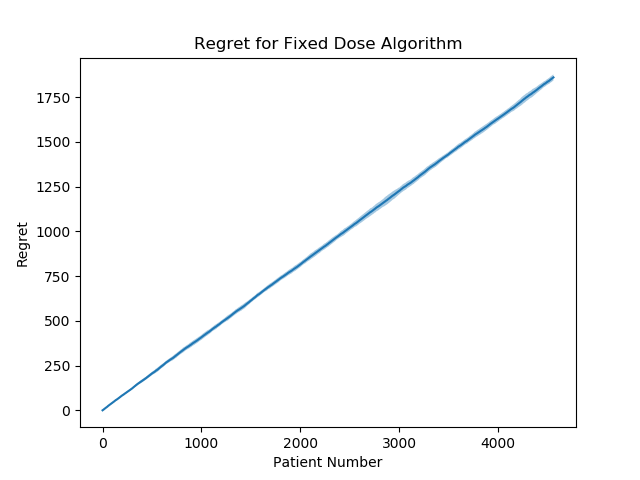
\includegraphics[width=\columnwidth]{regret_fd}
    \caption{Regret of the fixed dose algorithm}
    \label{fig:regret_fd}
\end{figure}

\begin{figure}
    \centering
    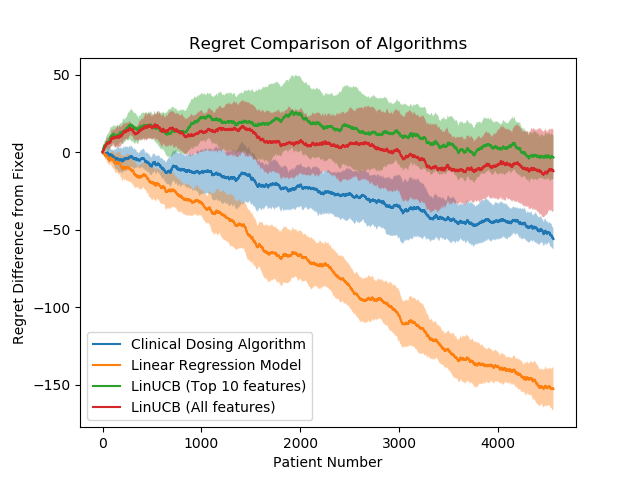
\includegraphics[width=\columnwidth]{regret}
    \caption{Regret of comparison algorithms with Fixed-Dose regret subtracted}
    \label{fig:regret}
\end{figure}

\begin{figure}
    \centering
    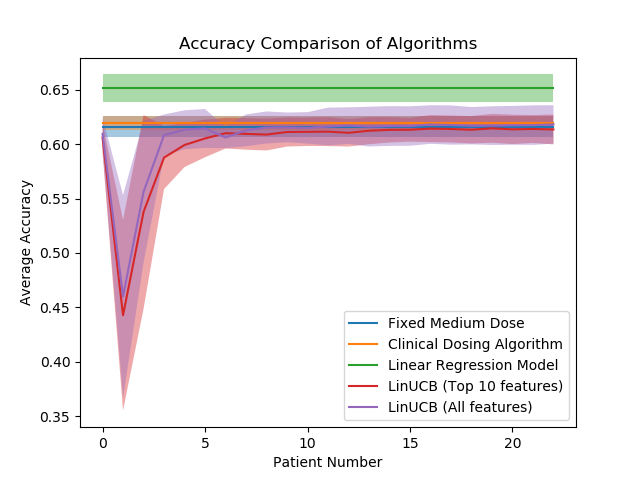
\includegraphics[width=\columnwidth]{accuracy}
    \caption{Accuracy of comparison algorithms  vs. the number of patients seen (multiply by 200 to get number of patients)}
    \label{fig:accuracy}
\end{figure}


Lastly, we consider the severity of the mistakes made by each of the algorithms. The accuracy and severity of mistakes is reported in \cref{severity-table}. We can first see that the fixed dose algorithm never makes a severe mistake because it always chooses the medium dose option, but it has the lowest accuracy. The clinical dosing algorithm has relatively good accuracy but suffers 5 severe mistakes in the dataset. The LinUCB with a binary reward function has good accuracy but suffers 23 mistakes, way more than any of the other algorithms, likely due to the exploration process early in the learning procedure. But, if the reward function is modified to use the wager reward, severity reward or severity + wager reward, the number of severity mistakes drops to 1. The accuracy also takes a hit but only by about 0.012-0.013 depending on the reward function, and still outperforms the fixed dose algorithm. The linear regression algorithm, despite having high accuracy, also suffers a significant number of severe mistakes.

\begin{table}[t]
\caption{Algorithm accuracy on entire dataset}
\label{severity-table}
\vskip 0.15in
\begin{center}
\begin{small}
\begin{sc}
\begin{tabular}{lcc}
\toprule
 &  & Severe\\
Algorithm & Accuracy & Errors \\
\midrule
Fixed Dose (35 mg/week)    & 0.612 & 0  \\
Clinical Dosing Algorithm  &  0.673 & 5  \\
\quad (Ignore NaN rows) & &\\
Clinical Dosing Algorithm  & 0.622 & 5 \\
\quad (Use 35 mg/week) & \\

LinUCB  (All features)  & 0.628 & 23 \\
\quad w/ binary reward & & \\

LinUCB  (All features)  & 0.615 & 1 \\
\quad w/ wager reward & & \\

LinUCB  (All features)  & 0.615 & 1 \\
\quad w/ severity reward & & \\

LinUCB  (All features)  & 0.616 & 1 \\
\quad w/ wager + severity reward & & \\

Linear Regression & 0.647 & 9\\
\bottomrule
\end{tabular}
\end{sc}
\end{small}
\end{center}
\vskip -0.1in
\end{table}



\section{Conclusions}
\label{conclusions}

This work has shown that it is feasible to construct an online learning algorithm to determine the correct dosing of Warfarin based on patient demographics, clinical data and genetic information. It was also shown that modifications to the reward function can successfully reduce the number of severe mistakes that the algorithm makes. In the future the following topics should be addressed

\begin{itemize}
    \item Attempt a nonlinear model (such as a neural network) to compare performance to linear models and to alleviate the problem of missing data.
    \item Try other bandit algorithms such as Thompson sampling to see if linear-regression levels of performance can be obtained by an online algorithm.
    \item Compare algorithms for different dosing bin strategies (like using 5 bins instead of 3) to see how number of options effects performance.
\end{itemize}


\bibliography{CS234_FinalReport}
\bibliographystyle{icml2018}


\end{document}


% This document was modified from the file originally made available by
% Pat Langley and Andrea Danyluk for ICML-2K. This version was created
% by Iain Murray in 2018. It was modified from a version from Dan Roy in
% 2017, which was based on a version from Lise Getoor and Tobias
% Scheffer, which was slightly modified from the 2010 version by
% Thorsten Joachims & Johannes Fuernkranz, slightly modified from the
% 2009 version by Kiri Wagstaff and Sam Roweis's 2008 version, which is
% slightly modified from Prasad Tadepalli's 2007 version which is a
% lightly changed version of the previous year's version by Andrew
% Moore, which was in turn edited from those of Kristian Kersting and
% Codrina Lauth. Alex Smola contributed to the algorithmic style files.
